% Options for packages loaded elsewhere
\PassOptionsToPackage{unicode}{hyperref}
\PassOptionsToPackage{hyphens}{url}
%
\documentclass[
]{article}
\usepackage{amsmath,amssymb}
\usepackage{iftex}
\ifPDFTeX
  \usepackage[T1]{fontenc}
  \usepackage[utf8]{inputenc}
  \usepackage{textcomp} % provide euro and other symbols
\else % if luatex or xetex
  \usepackage{unicode-math} % this also loads fontspec
  \defaultfontfeatures{Scale=MatchLowercase}
  \defaultfontfeatures[\rmfamily]{Ligatures=TeX,Scale=1}
\fi
\usepackage{lmodern}
\ifPDFTeX\else
  % xetex/luatex font selection
\fi
% Use upquote if available, for straight quotes in verbatim environments
\IfFileExists{upquote.sty}{\usepackage{upquote}}{}
\IfFileExists{microtype.sty}{% use microtype if available
  \usepackage[]{microtype}
  \UseMicrotypeSet[protrusion]{basicmath} % disable protrusion for tt fonts
}{}
\makeatletter
\@ifundefined{KOMAClassName}{% if non-KOMA class
  \IfFileExists{parskip.sty}{%
    \usepackage{parskip}
  }{% else
    \setlength{\parindent}{0pt}
    \setlength{\parskip}{6pt plus 2pt minus 1pt}}
}{% if KOMA class
  \KOMAoptions{parskip=half}}
\makeatother
\usepackage{xcolor}
\usepackage[margin=1in]{geometry}
\usepackage{graphicx}
\makeatletter
\def\maxwidth{\ifdim\Gin@nat@width>\linewidth\linewidth\else\Gin@nat@width\fi}
\def\maxheight{\ifdim\Gin@nat@height>\textheight\textheight\else\Gin@nat@height\fi}
\makeatother
% Scale images if necessary, so that they will not overflow the page
% margins by default, and it is still possible to overwrite the defaults
% using explicit options in \includegraphics[width, height, ...]{}
\setkeys{Gin}{width=\maxwidth,height=\maxheight,keepaspectratio}
% Set default figure placement to htbp
\makeatletter
\def\fps@figure{htbp}
\makeatother
\setlength{\emergencystretch}{3em} % prevent overfull lines
\providecommand{\tightlist}{%
  \setlength{\itemsep}{0pt}\setlength{\parskip}{0pt}}
\setcounter{secnumdepth}{5}
\usepackage{pdfpages}
\usepackage{fancyhdr}
\pagestyle{fancy}
\fancyhf{}
\fancyfoot[C]{\thepage}
\renewcommand{\headrulewidth}{0pt}
\setlength{\headheight}{15pt}
\usepackage[spanish]{babel}
\usepackage{booktabs}
\usepackage{longtable}
\usepackage{array}
\usepackage{multirow}
\usepackage{wrapfig}
\usepackage{float}
\usepackage{colortbl}
\usepackage{pdflscape}
\usepackage{tabu}
\usepackage{threeparttable}
\usepackage{threeparttablex}
\usepackage[normalem]{ulem}
\usepackage{makecell}
\usepackage{xcolor}
\ifLuaTeX
  \usepackage{selnolig}  % disable illegal ligatures
\fi
\IfFileExists{bookmark.sty}{\usepackage{bookmark}}{\usepackage{hyperref}}
\IfFileExists{xurl.sty}{\usepackage{xurl}}{} % add URL line breaks if available
\urlstyle{same}
\hypersetup{
  hidelinks,
  pdfcreator={LaTeX via pandoc}}

\author{}
\date{\vspace{-2.5em}}

\begin{document}

\newpage
\thispagestyle{empty}
\vspace*{2.5cm}
\begin{center}
\textbf{\Huge Evaluación de Bolsa Familia}
\vspace{1.5cm}

\vspace{1.5cm}
{\Large Proyecto Final de Tópicos de Políticas Públicas II}
\vspace{0.5cm}

\vspace{0.5cm}
\Large Guillermo Naranjo, Rodolfo Gloria, Sebastian Dulong y Javier Nieto
\vspace{1.5cm}


\includegraphics[width=6cm]{itam.png}

\vfill
15 de mayo del 2023
\end{center}
\newpage
\tableofcontents
\listoftables
\newpage

\hypertarget{bolsa-familia}{%
\section{Bolsa Familia}\label{bolsa-familia}}

El Programa Bolsa Familia (PBF) es un programa de transferencias
monetarias que tiene como fin apoyar a las familias en condición de
pobreza o pobreza extrema, esto se hace mediante transferencias que
buscan tener un impacto positivo en los niveles de salud y educación de
los beneficiarios. El programa fue implementado por el gobierno de
Brasil en Octube de 2003 y gracias a el éxito observado ha sido elogiado
por reducir la pobreza y la desigualdad en Brasil, y se ha expandido con
el paso de los años para incluir a más personas.En junio de 2015, cerca
del 25\% de la población brasileña, es decir, 13,827,369 familias, se
habían beneficiado del PBF. A pesar de su gran alcance, el programa
tiene un impacto financiero moderado en el presupuesto del país, ya que
representa solo el 0.45\% del Producto Interno Bruto brasileño.

PBF ha sido ampliamente reconocido como una estrategia exitosa en la
lucha contra el hambre y la pobreza en Brasil. En 2014, la Organización
de las Naciones Unidas para la Alimentación y la Agricultura (FAO)
destacó el papel del programa en la reducción de la inseguridad
alimentaria y la pobreza extrema en el país. Según la FAO, el programa
ha sido crucial para mejorar el acceso a alimentos para las poblaciones
más vulnerables, especialmente las mujeres y los niños.

\hypertarget{eligibilidad}{%
\subsection{Eligibilidad}\label{eligibilidad}}

Para ser elegibles, las familias deben tener ingresos mensuales
inferiores a 154 reales por persona (alrededor de \$550 pesos mexicanos
a mayo de 2023). Es importante destacar que se considera ``familia'' a
una unidad básica que puede estar compuesta por individuos con o sin
parentesco que comparten una misma vivienda. De esta manera, el programa
se enfoca en ayudar a las personas que se encuentran en una situación
vulnerable y requieren de apoyo financiero para cubrir sus necesidades
básicas.

El número de familias que pueden ingresar al Programa Bolsa Familia en
cada municipio está limitado por una estimación previa del número de
familias pobres en el área. Esta estimación se realiza a partir de los
datos del Censo Demográfico y de la Encuesta Nacional por Muestras de
Domicilios, ambos ejecutados por el Instituto Brasileño de Geografía y
Estadística (IBGE).

El acceso al Programa Bolsa Familia comienza con las familias
consideradas prioritarias, como las familias quilombolas (pertenecientes
a antiguas comunidades de afro-brasileros), familias indígenas, familias
que obtienen sus ingresos del reciclaje de basura o familias en las que
se ha identificado tanto trabajo infantil como situaciones análogas a
esclavitud. Estas familias tienen un acceso garantizado,
independientemente de si se ha alcanzado o no el límite municipal.
Después de asignar cupos a estas familias prioritarias, se asignan los
cupos restantes a las familias con menor ingreso mensual por persona.
Cuando hay paridad de ingresos, se priorizan las familias con mayor
número de niños y adolescentes menores de 18 años.

Las familias podrían perder su vinculación con el programa en caso de:

\begin{enumerate}
\def\labelenumi{\arabic{enumi}.}
\tightlist
\item
  No cumplen de manera repetitiva con los requisitos de salud y
  educación.
\item
  Superen la línea de pobreza debido a un aumento de sus ingresos.
\item
  No actualicen su información en el Cadastro Único.
\end{enumerate}

Cuando una familia sobrepasa la línea de pobreza pero sigue por debajo
de medio salario mínimo mensual per cápita, no se les cancelan las
transferencias inmediatamente. En su lugar, se les extienden los
beneficios por dos años para garantizar que las mejoras económicas sean
sostenibles. Luego de este plazo, se reevalúa la situación de la familia
y, si sus ingresos siguen por encima de los límites del programa o la
familia no actualiza su información, se cancelan los beneficios. Si una
familia desea desvincularse voluntariamente del programa, puede hacerlo
y, en caso de que sus ingresos disminuyan de nuevo, tiene derecho a
volver al programa dentro de los 36 meses siguientes.

\hypertarget{transferencias}{%
\subsection{Transferencias}\label{transferencias}}

Existen cuatro tipos de transferencias que varían según la situación y
composición de cada familia:

\begin{itemize}
\item
  Beneficio básico: consiste en la entrega de 77 reales mensuales y está
  dirigido exclusivamente a familias que se encuentran en extrema
  pobreza en Brasil, lo que significa que su ingreso mensual por persona
  es menor a 77 reales. Este beneficio es independiente de la
  composición familiar y puede ser recibido incluso si no hay individuos
  menores de 18 años.
\item
  Beneficio variable: consiste en la entrega de 35 reales y está
  destinado a las familias en situación de pobreza o extrema pobreza que
  tienen mujeres embarazadas o en etapa de lactancia, así como también
  niños y adolescentes de hasta 15 años en su composición familiar. Cada
  familia puede recibir hasta cinco beneficios variables, uno por cada
  individuo elegible.
\item
  Beneficio variable joven: consiste en la entrega de 42 reales y está
  destinado a las familias en situación de pobreza o extrema pobreza que
  tienen jóvenes de entre 16 y 17 años en su composición familiar. Cada
  familia puede recibir hasta dos beneficios variables jóvenes. Este
  beneficio se otorga hasta el mes de diciembre del año en que el
  adolescente cumple 18 años.
\item
  Beneficio superación de la pobreza: es una ayuda financiera adicional
  del Programa Bolsa Familia y está destinado a las familias que, a
  pesar de recibir los demás beneficios correspondientes a su
  composición familiar, todavía no logran superar la línea de extrema
  pobreza. Este beneficio se otorga de manera personalizada para cada
  situación familiar y se calcula para que la familia pueda alcanzar los
  77 reales por persona.
\end{itemize}

\newpage

\hypertarget{datos-y-anuxe1lisis-estaduxedstico}{%
\section{Datos y análisis
estadístico}\label{datos-y-anuxe1lisis-estaduxedstico}}

El análisis de impacto del Programa Bolsa Familia de Brasil se basa en
una amplia base de datos que abarca 27 estados y 5,283 municipios en los
que se implementó el programa. La disponibilidad de estas cifras permite
una evaluación detallada del desempeño del programa en cada uno de los
municipios. Entre las variables disponibles para el análisis se
encuentran: el número de familias beneficiadas, el número de alumnos
beneficiados, la tasa de cobertura, la tasa de cobertura de población en
extrema pobreza, la tasa de deserción escolar, el desempeño en educación
primaria y secundaria, y el Índice de Desarrollo Humano, desglosado en
sus componentes de educación, ingresos y longevidad (salud). Estos datos
permiten evaluar el impacto del programa en las dimensiones de educación
y salud, lo que a su vez permitirá una comprensión más completa de su
efectividad en la lucha contra la pobreza y la desigualdad en Brasil.

\begin{table}[!h]

\caption{\label{tab:unnamed-chunk-1}Descripción de variables}
\centering
\fontsize{8}{10}\selectfont
\begin{tabular}[t]{ll}
\toprule
Variable & Descripcion\\
\midrule
pc\_pbf\_pop & Porcentaje de población del PBF en el municipio\\
pc\_alunosPBF & Porcentaje de alumnos del municipio que participan en PBF\\
acomp\_freq & Tasa de seguimiento de la condicionalidad de la asistencia escolar (6 a 15 años)\\
ab\_ef & Tasa de deserción en la escuela primaria - 0 a 100\\
ap\_ef & Tasa de aprobación en la escuela primaria\\
\addlinespace
cobalvopbf & Porcentaje de cobertura del público objetivo del PBF Fundamental\\
porteIBGE & Tamaño del municipio - población\\
rdpc\_2010 & Renta per cápita según Censo 2010\\
infraescolar\_em\_2011 & Indicador de infraestructura de las escuelas de EM en el municipio - continuo\\
infraescolar\_ef\_2011 & Indicador de infraestructura de las escuelas de EF en el municipio - continuo\\
\addlinespace
propextpobre\_2010 & Proporción de la población extremadamente pobre\\
rep\_ef & Tasa de fracaso en la escuela primaria\\
rep\_em & Tasa de fracaso en la escuela primaria\\
tesouro & Transferencias totales del tesoro nacional\\
est\_fam\_PBF\_2006 & Estimación de familias PBF - 2006 (Hasta 140.00 renta per cápita)\\
\addlinespace
est\_fam\_PBF\_2010 & Estimación de familias PBF - 2010 (Hasta 140.00 renta per cápita)\\
ano & Año de la estimación\\
agua\_esgoto\_inadeq\_2010 & Porcentaje de personas en hogares con suministro de agua y alcantarillado inadecuados\\
pc\_lixo\_2010 & Porcentaje de población en viviendas con recolección de basura\\
pc\_luz\_2010 & Porcentaje de población en hogares con electricidad\\
\addlinespace
PIBcapita & PIB municipal por capita\\
PIB & PIB municipal\\
IDHM\_E\_2010 & IDH-M en 2010 - educación\\
IDHM\_L\_2010 & IDH-M en 2010 - longevidad\\
IDHM\_R\_2010 & IDH-M en 2010 - ingresos\\
\addlinespace
pbf\_capita & Valor de transferencias PBF per cápita\\
alunospbf & Número de alumnos en PBF\\
fam\_pbf & Número de familias beneficiarias de PBF\\
pbf\_valor & Valor de transferencias PBF\\
PIB\_agropec & PIB del sector agropecuario del municipio\\
\addlinespace
PIB\_servicios & PIB del sector servicios del municipio\\
PIB\_industria & PIB de las industrias del municipio\\
nome\_municipio & Nombre del municipio\\
\bottomrule
\end{tabular}
\end{table}

\begin{table}[!h]

\caption{\label{tab:unnamed-chunk-3}Resumen de las variables}
\centering
\fontsize{8}{10}\selectfont
\begin{tabular}[t]{lcccccc}
\toprule
  & Min & 1st Qu & Mediana & Media & 3rd Qu & Max\\
\midrule
X..pc\_pbf\_pop & 0.18 & 18.32 & 32.68 & 34.87 & 51.43 & 108.31\\
X..acomp\_freq & 29.73 & 86.37 & 91.55 & 89.89 & 95.13 & 100.00\\
X....ab\_ef & 0.00 & 0.98 & 2.26 & 3.08 & 4.37 & 40.23\\
X....ap\_ef & 44.90 & 81.19 & 87.33 & 86.20 & 92.30 & 100.00\\
X..cobalvopbf & 1.56 & 89.05 & 104.82 & 102.78 & 117.24 & 727.59\\
\addlinespace
X..porteibge & 0.00 & 1.00 & 2.00 & 1.78 & 3.00 & 6.00\\
X..rdpc\_2010 & 96.25 & 281.12 & 467.65 & 493.61 & 650.62 & 2,043.74\\
infraescolar\_ef\_2011 & 35.75 & 52.49 & 56.12 & 55.72 & 59.11 & 72.34\\
infraescolar\_em\_2011 & 36.53 & 55.92 & 60.21 & 60.02 & 63.35 & 72.34\\
propextpobre\_2010 & 0.00 & 0.03 & 0.08 & 0.13 & 0.22 & 0.67\\
\addlinespace
X....rep\_ef & 0.00 & 6.10 & 10.07 & 10.71 & 14.53 & 41.93\\
X....rep\_em & 0.00 & 4.31 & 7.97 & 9.15 & 12.73 & 55.84\\
X...tesouro & 0.00 & 5,348,000.00 & 8,324,000.00 & 16,590,000.00 & 15,890,000.00 & 2,836,000,000.00\\
est\_fam\_pbf\_2006 & 30.00 & 439.80 & 989.00 & 2,335.60 & 2,188.50 & 327,188.00\\
est\_fam\_pbf\_2010 & 5.00 & 411.00 & 1,008.00 & 2,469.00 & 2,341.00 & 500,686.00\\
\addlinespace
X.....ano & 2,008.00 & 2,009.00 & 2,010.00 & 2,010.00 & 2,011.00 & 2,012.00\\
agua\_esgoto\_inadeq\_2010 & 0.00 & 0.53 & 3.26 & 9.20 & 13.02 & 85.36\\
X.pc\_lixo\_2010 & 0.00 & 93.72 & 98.03 & 94.05 & 99.49 & 100.00\\
X.pc\_luz\_2010 & 27.41 & 97.65 & 99.39 & 97.19 & 99.87 & 100.00\\
X..pibcapita & 1.72 & 5.11 & 9.37 & 12.50 & 15.17 & 387.17\\
\addlinespace
X.....pib & 4,957.00 & 43,141.00 & 90,146.00 & 658,679.00 & 231,714.00 & 477,005,597.00\\
X.idhm\_e\_2010 & 0.21 & 0.49 & 0.56 & 0.56 & 0.63 & 0.82\\
X.idhm\_l\_2010 & 0.67 & 0.77 & 0.81 & 0.80 & 0.84 & 0.89\\
X.idhm\_r\_2010 & 0.40 & 0.57 & 0.65 & 0.64 & 0.71 & 0.89\\
X..pbf\_capita & 58.67 & 265.39 & 309.52 & 315.01 & 360.38 & 1,206.40\\
\addlinespace
X..alunospbf & 0.00 & 562.00 & 1,345.00 & 3,215.00 & 3,187.00 & 332,119.00\\
X...fam\_pbf & 1.00 & 406.00 & 980.00 & 2,263.00 & 2,273.00 & 228,078.00\\
X.pc\_alunospbf & 1.12 & 41.16 & 63.07 & 62.86 & 85.68 & 262.65\\
pib\_industria & 282.00 & 3,875.00 & 9,572.00 & 155,256.00 & 38,916.00 & 76,857,507.00\\
X.pib\_servicos & 4,132.00 & 23,964.00 & 49,008.00 & 376,566.00 & 120,427.00 & 309,794,582.00\\
\addlinespace
X.pib\_agropec & 0.00 & 7,349.00 & 16,631.00 & 31,136.00 & 35,500.00 & 832,783.00\\
nome\_municipio & 27,825.00 & NA & NA & NA & NA & NA\\
X..cobalvopbf.1 & 1.56 & 89.05 & 104.82 & 102.78 & 117.24 & 727.59\\
X..pbf\_valor & 660.00 & 437,378.00 & 1,121,632.00 & 2,729,793.00 & 2,745,678.00 & 317,886,792.00\\
\bottomrule
\end{tabular}
\end{table}
\newpage

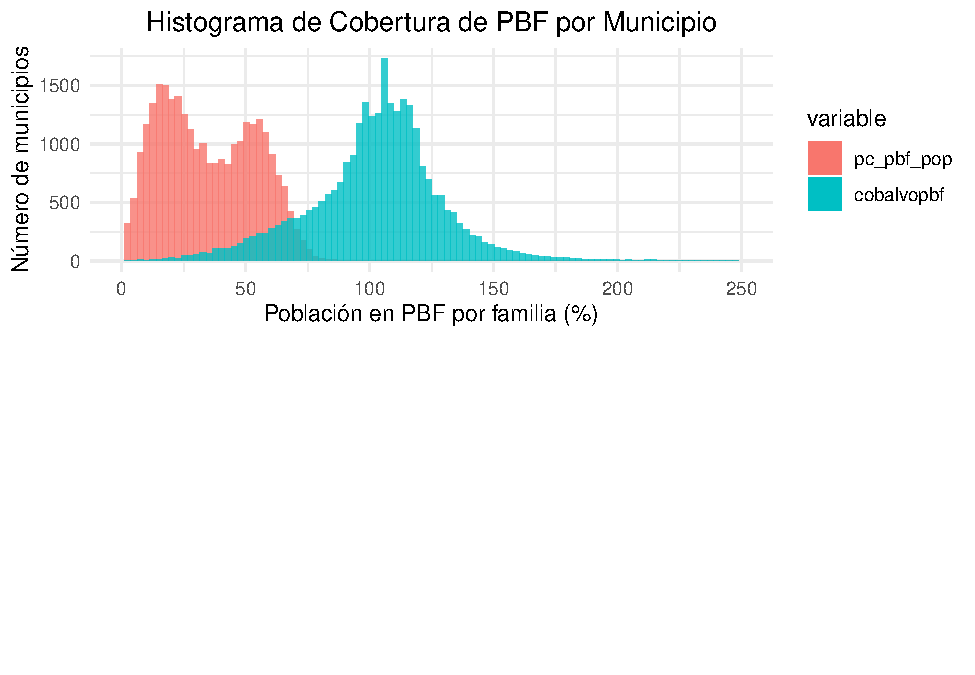
\includegraphics{PBF_files/figure-latex/unnamed-chunk-4-1.pdf}

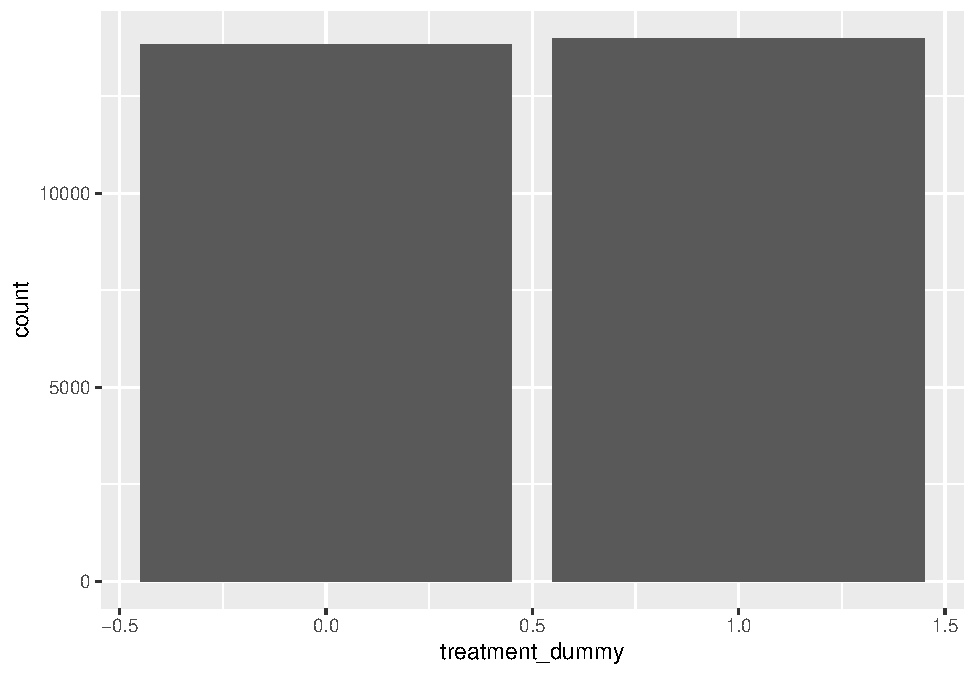
\includegraphics{PBF_files/figure-latex/unnamed-chunk-5-1.pdf}

\newpage

\hypertarget{efectos-fijos}{%
\section{Efectos Fijos}\label{efectos-fijos}}

La evaluación rigurosa del programa Bolsa Familia a nivel municipal es
esencial para comprender su efectividad y determinar su impacto en la
reducción de la pobreza y la promoción de la inclusión social. En este
sentido, la regresión de efectos fijos con datos de panel se destaca
como una valiosa herramienta de análisis. Esta técnica permite controlar
por factores no observados, como características socioeconómicas y
culturales específicas de cada municipio, que podrían influir en los
resultados del programa. Al incluir los efectos fijos municipales en el
modelo de regresión, se elimina la influencia de estos factores
constantes a lo largo del tiempo, lo que proporciona una estimación más
precisa del impacto real de Bolsa Familia en cada contexto local.

Se utilizará la regresión de efectos fijos para examinar el impacto de
factores específicos en la salud, la educación y la pobreza en cada
municipio. Mediante la inclusión de efectos fijos municipales en el
análisis, se controlará por características propias de cada municipio
que permanecen constantes a lo largo del tiempo. Esto nos permitirá
determinar de manera más precisa cómo variables como la inversión en
infraestructura, el acceso a servicios educativos, los indicadores de
salud, el nivel de ingresos y otros factores relevantes influyen en los
resultados relacionados con la salud, la educación y la pobreza.

\begin{enumerate}
\def\labelenumi{\arabic{enumi}.}
\item
  Índice de Deserción Escolar: El índice de deserción escolar es un
  indicador clave para medir la capacidad del programa para retener a
  los estudiantes en el sistema educativo. Un índice de deserción
  escolar más bajo sugiere que el programa está logrando reducir la tasa
  de abandono escolar, lo cual es esencial para garantizar que los
  estudiantes beneficiarios puedan completar su educación y tener
  mayores oportunidades en el futuro.
\item
  PIB per cápita: Esta variable permite evaluar el impacto del programa
  en el bienestar económico de los beneficiarios y en la reducción de la
  pobreza. Un incremento en el el PIB per cápita indicaría que el
  programa está logrando mejorar las condiciones económicas de las
  familias beneficiarias, lo cual es un objetivo central de Bolsa
  Familia.
\item
  Índice de Desarrollo Humano relacionado con la Salud: El índice de
  desarrollo humano relacionado con la salud es esencial para evaluar
  cómo el programa contribuye a mejorar el acceso a servicios de salud y
  promover una mejor calidad de vida. Un aumento en este índice
  indicaría que el programa está impactando positivamente en la salud de
  los beneficiarios, garantizando un acceso adecuado a servicios de
  atención médica y mejorando su bienestar general.
\end{enumerate}

En resumen, estas variables nos permitirán medir y evaluar el impacto
del programa Bolsa Familia en las tres áreas clave: salud, educación e
ingresos. El análisis de estas variables proporcionará información
valiosa sobre cómo el programa está contribuyendo al mejoramiento de la
salud de los beneficiarios, su rendimiento educativo y su bienestar
económico.

\newpage
\begin{table}[!htbp] \centering 
  \caption{Resumen de los modelos} 
  \label{} 
\begin{tabular}{@{\extracolsep{5pt}}lccc} 
\\[-1.8ex]\hline 
\hline \\[-1.8ex] 
 & \multicolumn{3}{c}{\textit{Variable dependiente:}} \\ 
\cline{2-4} 
\\[-1.8ex] & Deserción escolar & PIB capita & IDH longevidad \\ 
\\[-1.8ex] & (1) & (2) & (3)\\ 
\hline \\[-1.8ex] 
 cobalvopbf & $-$0.077$^{***}$ & 0.033$^{***}$ & 0.044$^{***}$ \\ 
  & ($-$0.087, $-$0.067) & (0.026, 0.040) & (0.040, 0.047) \\ 
  & & & \\ 
 pc\_pbf\_pop & $-$0.118$^{***}$ & $-$0.046$^{***}$ & $-$0.359$^{***}$ \\ 
  & ($-$0.147, $-$0.089) & ($-$0.066, $-$0.026) & ($-$0.370, $-$0.348) \\ 
  & & & \\ 
 pc\_alunospbf & 0.372$^{***}$ & $-$0.211$^{***}$ & $-$0.218$^{***}$ \\ 
  & (0.345, 0.400) & ($-$0.230, $-$0.192) & ($-$0.228, $-$0.208) \\ 
  & & & \\ 
 pbf\_valor & $-$0.100$^{***}$ & $-$0.094$^{***}$ & 0.036$^{***}$ \\ 
  & ($-$0.124, $-$0.076) & ($-$0.111, $-$0.077) & (0.027, 0.045) \\ 
  & & & \\ 
 pbf\_capita & $-$0.135$^{***}$ & 0.093$^{***}$ & 0.019$^{***}$ \\ 
  & ($-$0.143, $-$0.127) & (0.087, 0.098) & (0.017, 0.022) \\ 
  & & & \\ 
 porteibge & 0.047$^{***}$ & $-$0.001 & 0.019$^{***}$ \\ 
  & (0.020, 0.074) & ($-$0.019, 0.018) & (0.009, 0.029) \\ 
  & & & \\ 
 pib\_industria & $-$0.062$^{**}$ & 1.475$^{***}$ & 0.058$^{***}$ \\ 
  & ($-$0.109, $-$0.014) & (1.442, 1.508) & (0.040, 0.075) \\ 
  & & & \\ 
 pib\_servicos & 0.108$^{***}$ & $-$0.723$^{***}$ & $-$0.045$^{***}$ \\ 
  & (0.042, 0.174) & ($-$0.769, $-$0.677) & ($-$0.069, $-$0.021) \\ 
  & & & \\ 
 pib\_agropec & $-$0.063$^{***}$ & 0.213$^{***}$ & 0.041$^{***}$ \\ 
  & ($-$0.085, $-$0.041) & (0.197, 0.228) & (0.032, 0.049) \\ 
  & & & \\ 
\hline \\[-1.8ex] 
Observaciones & 27,795 & 27,820 & 27,820 \\ 
R$^{2}$ & 0.117 & 0.359 & 0.442 \\ 
R$^{2}$ Ajustada & $-$0.091 & 0.208 & 0.312 \\ 
Estadístico F & 331.368$^{***}$ (df = 9; 22504) & 1,398.981$^{***}$ (df = 9; 22529) & 1,986.522$^{***}$ (df = 9; 22529) \\ 
\hline 
\hline \\[-1.8ex] 
\textit{Nota:}  & \multicolumn{3}{r}{$^{*}$p$<$0.1; $^{**}$p$<$0.05; $^{***}$p$<$0.01} \\ 
\end{tabular} 
\end{table}

\hypertarget{resultados}{%
\subsection{Resultados}\label{resultados}}

\newpage

\hypertarget{matching}{%
\section{Matching}\label{matching}}

Para la evaluación de Bolsa Familia, nos enfrentamos con el problema de
no tener una variable de tratamiento como tal. Es decir, no teníamos
forma de conseguir los datos de cada estudiante de Brasil, y si
participó o no en el programa. De alguna forma, necesitamos esto para
poder comparar entre un grupo de tratamiento y uno de control, y poder
aplicar con esta información distintos modelos que nos digan el impacto
de la política pública.

Ante este problema, usamos Matching, un método que nos permite asociar
municipios a clusters (o grupos) con los que comparten similitudes,
conteniendo una proporción similar de municipios tratados y no tratados.
Entonces, se necesita una variable de tratamiento y variables que sirvan
como covariadas para poder relacionar municipios entre sí que tengan
probabilidades similares de ser tratados. A esto, le llamaremos puntaje
de propensión. El matching se realizaría con todos los municipios
únicamente del 2008, año de inicio del dataset, para poder llevar un
rastreo de su desempeño a lo largo de 4 años.

\hypertarget{variable-de-tratamiento}{%
\subsection{Variable de tratamiento}\label{variable-de-tratamiento}}

Pero, ¿cómo conseguimos una variable de tratamiento? Para esto, reunimos
las siguientes variables con datos anuales por cada uno de los
municipios:

\begin{itemize}
\tightlist
\item
  pc\_pbf\_pob: porcentaje de la población que participa en PBF del
  municipio
\item
  covalbopbf: porcentaje de cobertura del público objetivo del PBF
  fundamental
\item
  pc\_alunospbf: porcentaje de alumnos del municipio en PBF
\end{itemize}

De este modo, asignamos con un 0 (no tratados) a aquellos municipios que
no superaran la mediana de la muestra total de todos los municipios
registrados en 2008 para las tres variables, y con un 1 a los que sí.
Para esto, se excluyó una muestra considerablemente pequeña de
municipios que no contaban con información suficiente para ser
participar en el matching.

\hypertarget{covariadas}{%
\subsection{Covariadas}\label{covariadas}}

Para las variables covariadas que nos ayuden a enconrtar similitudes
entre los municipios, usamos las siguientes 4, que creemos dan una
imagen general de la situación y contexto de cada municipio:

\begin{itemize}
\tightlist
\item
  portel\_IBGE: tamaño del municipio (población)
\item
  PIB\_agropec: PIB agropecuario municipal del año
\item
  PIB\_servicos: PIB del sector servicios municipal del año
\item
  PIB\_industria: PIB de la industria del municipio del año
\end{itemize}

Finalmente, se hizo el proceso de matching con la librería de MatchIt de
R, usando el método de K-vecinos cercanos, con n= 1. Es decir, por cada
municipio tratado, se le asignó un municipio de características
similares, pero con tratamiento por debajo de la mediana.

Antes del matching, se empezó con un total de 5565 municipios, y tras
haber terminado este proceso, quedamos con un total de 5475, lo cual
sigue siendo una muestra muy completa.

A continuación, mostramos las gráficas de la distribución del puntaje de
propensión antes y después de hacer matching. Se puede apreciar que
ambas distribuciones son extremadamente similares. En un trabajo de
Aprendizaje de Máquina, esto nos preocuparía, ya que nos indicaría que
nuestro modelo está sobreajustado. No obstante, en este contexto es muy
favorable. Como usamos K-vecinos cercanos únicamente para encontrar
municipios parecidos a los tratados, pero sin tratamiento, y no para
predecir a qué categoría pertenecerían nuevos municipios, el modelo
funcionó perfectamente. Es decir, los municipios tratados y los no
tratados tienen muy alta similitud, lo cual nos ayudará a medir los
efectos del programa de muy buena manera.

\begin{center}\includegraphics{PBF_files/figure-latex/unnamed-chunk-8-1} \end{center}

La siguiente gráfica nos muestra mejor los resultados anteriores,
colocando las funciones de densidad antes y después de Matching una
encima de la otra para ver las diferencias. Se puede apreciar que a
excepción de los puntajes casi cercanos a 0, tienen prácticamente la
misma función densidad.

\begin{center}\includegraphics{PBF_files/figure-latex/unnamed-chunk-9-1} \end{center}
\newpage

\newpage

\hypertarget{referencias}{%
\section{Referencias}\label{referencias}}

\begin{enumerate}
\def\labelenumi{\arabic{enumi}.}
\tightlist
\item
  \url{https://publications.iadb.org/publications/spanish/viewer/S\%C3\%ADntesis-del-programa-Bolsa-Familia-en-Brasil.pdf}
\end{enumerate}

\end{document}
